\documentclass[11pt]{article}

\usepackage[margin=1in]{geometry}
\usepackage{graphicx}
\usepackage{booktabs}
\usepackage{array}
\usepackage{amsmath}
\usepackage{amssymb}
\usepackage{microtype}
\usepackage{caption}
\usepackage[dvipsnames]{xcolor}
\usepackage[colorlinks=true,linkcolor=BrickRed,citecolor=BrickRed,urlcolor=RoyalBlue]{hyperref}

\captionsetup{font=small,labelfont=bf}
\graphicspath{{figs/}}

% let TeX stretch to avoid prose overflowing the margin
\setlength{\emergencystretch}{3em}

% consistent chemistry / units shortcuts
\newcommand{\coo}{CO\textsubscript{2}}
\newcommand{\kgmwh}{kg/MWh}

\title{\bfseries Carbon-optimal data-center siting is not robust to the
carbon-accounting choice: a specification-curve analysis on live grid data}

\author{Lakshay Mani\thanks{Northeastern University.
\href{mailto:mani.l@northeastern.edu}{mani.l@northeastern.edu}. Code and data:
\url{https://github.com/LakshayMani0406/gridpulse} (\texttt{gridpulse}, v0.2.0).}}

\date{July 2026\\[4pt]
\normalsize\itshape Draft preprint. Target: arXiv eess.SY / econ.EM.
Artifact: \texttt{gridpulse}, reproducible from zero.}

\begin{document}
\maketitle

\begin{abstract}
\noindent
The surge in data-center load has made ``where should the next data center go to
minimize carbon?'' a live policy question, usually answered by ranking regions on
a single emission factor. \textbf{Our single claim: that ranking---and therefore
the carbon-optimal siting recommendation---is not robust to the carbon-accounting
choice.} Using two years of hourly EIA-930 data for 27 US balancing authorities
(BAs) across all three interconnects, with the computed average factor validated
against EIA's own published hourly \coo{} to a median of 1.6\% for
fossil-dominated BAs, we compute a per-BA carbon factor under a \emph{multiverse}
of defensible accounting choices spanning four axes: temporal (short-run dispatch
vs long-run build margin), accounting boundary (production vs
consumption/import-adjusted), spatial resolution (BA vs nodal), and estimation
method (regression vs supply-side instrument vs capacity-expansion model). Across
six specifications, \textbf{24 of 27 BAs change siting rank and only 3 are robust}
(two Pacific-Northwest hydro BAs robustly green, one coal BA robustly dirty). The
re-rankings are not cosmetic: the median flipping BA moves 12 ranks, 10 BAs span
at least half the fleet, and four undergo outright inversions---Idaho Power (IPCO)
runs from rank 3 (near-greenest, short-run) to 25 (near-worst, long-run). The
short-run marginal factor is itself hard to identify: three independent
supply-side estimators converge within 20\% for only 6 of 23 BAs, which we read as
evidence \emph{for} the fragility thesis---the margin is genuinely ill-defined
outside a single-fossil-unit regime---not as validation. We turn the critique into
a decision rule: site where the verdict is robust across all accounting choices
(the Pacific-NW hydro core), or, where that core is unavailable, hedge across
regions whose rank vectors are anti-correlated (IPCO+MISO, rank-correlation
$-0.93$, caps worst-case rank at 9 versus 25 for either site alone). All numbers
regenerate from the released \texttt{gridpulse} pipeline.
\end{abstract}

\section{Introduction}

A new data center is an increment of load that persists for 15+ years. Its climate
impact is therefore governed by the grid's \textbf{marginal} response, not its
average---a point established since Siler-Evans et al.\ (2012). The policy
literature and commercial siting tools translate this into a ranking: order BAs by
a carbon factor, site in the low-carbon ones. \textbf{We show that ranking is not
robust.} ``The marginal factor'' hides four choices, each contested at the
research frontier and each capable of inverting which region is ``greenest'':

\begin{enumerate}
\item \textbf{Temporal horizon.} The short-run \emph{dispatch} margin (which
existing unit ramps) differs from the long-run \emph{build} margin (what new
capacity the load induces). Short-run-optimal operation can raise long-run
emissions (Gagnon \& Cole 2022); marginal factors have not fallen
as fast as average factors (Holland et al.\ 2022).
\item \textbf{Accounting boundary.} Production-based emissions ignore that a BA may
serve load with dirty imports; consumption-based (import-adjusted) accounting via
interchange flow-tracing (de Chalendar et al.\ 2019) re-ranks regions.
\item \textbf{Spatial resolution.} Two nodes in the same BA face different marginal
carbon under transmission congestion; BA-average erases this.
\item \textbf{Estimation method.} Regression (Siler-Evans), dispatch/instrumental
estimates, and capacity-expansion models (NREL Cambium) need not agree.
\end{enumerate}

Our contribution is a single, sharp claim answered with a specification-curve
(multiverse) analysis (Simonsohn, Simmons \& Nelson 2020): \textbf{a
carbon-optimal siting recommendation is meaningless without the accounting choice
that produced it, and the set of sites that are good under \emph{every} choice is
small.} We build and validate each method on live data, release the full pipeline
as \texttt{gridpulse}, and close with a decision rule that follows directly from
the fragility we measure.

\section{Data}

\begin{itemize}
\item \textbf{EIA-930 hourly} fuel mix, demand, and BA-to-BA interchange for 27
balancing authorities across all three interconnects, via the EIA API v2. 24
months at full coverage; 2019--present for a subset (Holland test). These 27 are a
\textbf{truncation of the $\sim$66-BA EIA interchange network} (see \S6).
\item \textbf{EIA Hourly Electric Grid Monitor} per-BA workbooks---EIA's
\emph{published} hourly \coo{}, used as validation ground truth (not
self-consistency).
\item \textbf{NREL Cambium} long-run marginal emission rates (LRMER), GEA-region
resolution, forward scenarios.
\item \textbf{CAISO OASIS} nodal LMP with congestion decomposition (no-auth,
reproducible), for the intra-BA nodal analysis.
\item \textbf{FracTracker} national data-center tracker (per-facility MW +
location).
\end{itemize}

\section{Methods}

\begin{itemize}
\item \textbf{AEF}: $\sum \coo / \sum \text{generation}$, on EIA's production basis
(fossil combustion only: COL, NG, OIL), validated against EIA's published hourly
\coo.
\item \textbf{Short-run MEF}: Siler-Evans OLS of $\Delta\coo$ on
$\Delta\text{demand}$ over consecutive hours, bootstrap CIs; recovers a planted
margin to machine precision on synthetic data.
\item \textbf{Consumption MEF}: emissions flow-tracing over the interchange network
(de Chalendar 2019 linear system), then a marginal factor on the import-adjusted
series. Runs on the 27-BA modeled subnetwork; imports across cut edges are dropped
(\S6).
\item \textbf{Supply-side instruments} (identification stress-test): (i)
VRE-ramp---carbon displaced per MWh of exogenous wind/solar with demand held flat;
(ii) generation-trip---emissions response to detected forced outages.
\item \textbf{Nodal LME}: CAISO nodal congestion component modulating the BA system
margin (directional only; exact nodal \kgmwh{} requires proprietary CEII shift
factors).
\item \textbf{Long-run}: NREL Cambium LRMER/SRMER, mapped GEA-region $\to$ BA.
\item \textbf{Specification curve}: rank BAs under every (temporal $\times$
accounting $\times$ spatial $\times$ method) combination; classify each BA
robust-green / robust-dirty / flips by its rank range across specifications.
\end{itemize}

\section{Results}

Generated by the live run (\texttt{gridpulse phase3}); tables in
\texttt{FINDINGS.md}/\texttt{EVIDENCE.md}, committed rank matrix in
\texttt{data/multiverse\_ranks.csv} and robustness classification in
\texttt{data/multiverse\_robustness.csv}.

\paragraph{4.1 Validation (of the pipeline, not the thesis).}
Computed AEF matches EIA's \emph{published} hourly \coo{} to a median of
\textbf{1.6\%} across fossil-dominated BAs using EIA's own per-fuel factors
(ERCO $-2.4\%$, MISO $-0.6\%$, DUK $-5.4\%$, SOCO $-1.5\%$; Figure~\ref{fig:val}).
This anchors the average-factor pipeline before any marginal analysis; it says
nothing about how well-identified the \emph{marginal} factor is (see 4.2).

\begin{figure}[t]
\centering
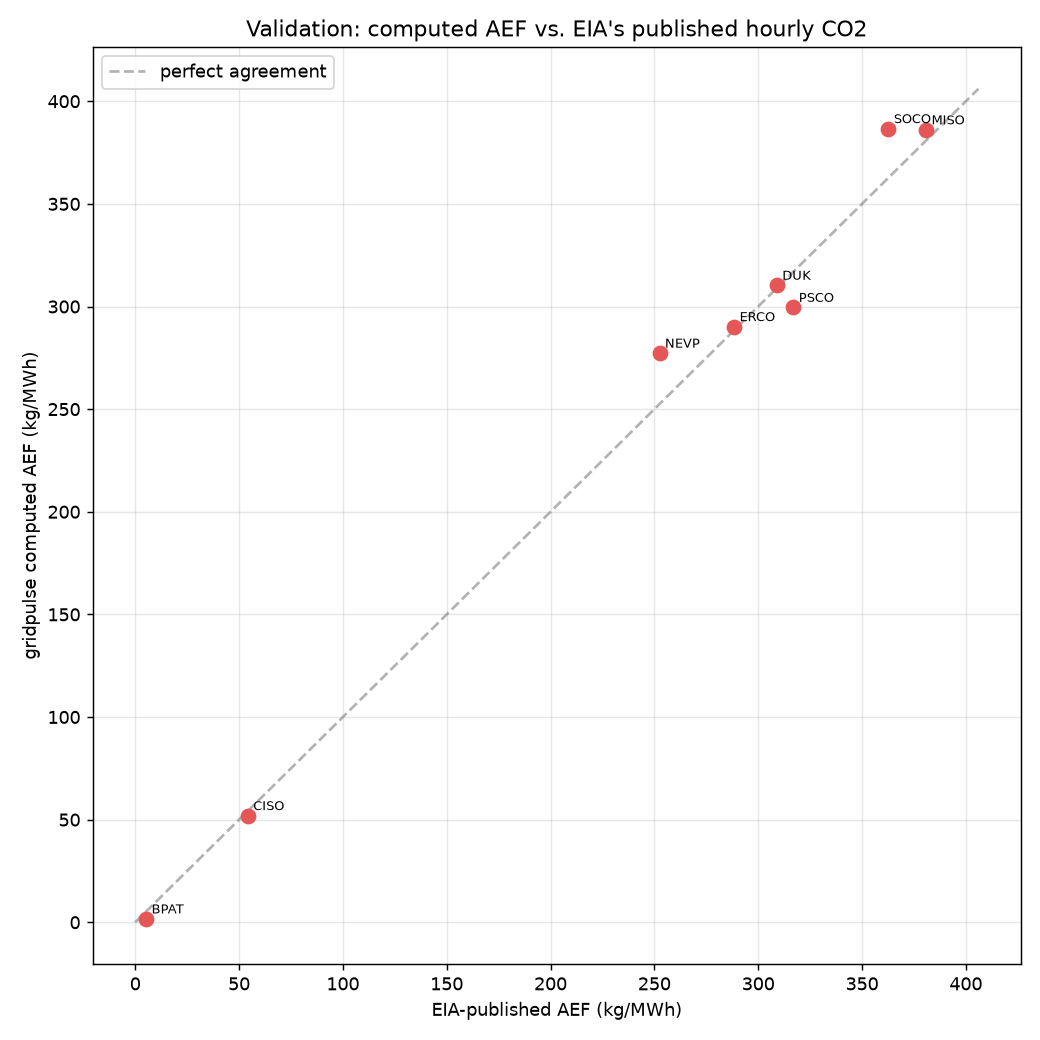
\includegraphics[width=0.62\textwidth]{validation_aef.png}
\caption{Computed AEF vs.\ EIA's published hourly \coo{} for fossil-dominated BAs.
Points hug the identity line (median deviation 1.6\%), anchoring the
average-factor pipeline before any marginal analysis.}
\label{fig:val}
\end{figure}

\paragraph{4.2 The short-run margin is hard to identify---evidence for fragility.}
Siler-Evans, the VRE-ramp instrument, and generation-trip events converge within
20\% for \textbf{only 6 of 23 BAs} (FPC, PJM, SWPP, SOCO, MISO, AZPS)---exactly
those where a single fossil unit sets the margin. In
storage/solar/import-heavy systems the three estimates diverge by 100--800\%
(CISO 141\%, WACM 573\%, NEVP 847\%), because batteries and imports break the
one-margin assumption. We do \textbf{not} read 6/23 as validation of the MEF. It
is direct evidence that the object the siting literature ranks on is genuinely
ill-defined for three-quarters of the fleet---a first-order reason the downstream
ranking is fragile.

\begin{figure}[t]
\centering

\includegraphics[width=0.85\textwidth]{aef_vs_mef.png}
\caption{Average (AEF) vs.\ short-run marginal (MEF) emission factor by BA. The
two orderings are visibly different---BAs clean on average are not the same set as
BAs clean on the margin---which is the raw material for the re-rankings in \S4.6.}
\label{fig:aefmef}
\end{figure}

\paragraph{4.3 Consumption re-ranking.}
Import-adjusted (flow-traced) marginal carbon moves several BAs 10+ ranks versus
production-based (CPLE $-14$, PGE $+11$, ISNE $-10$).

\paragraph{4.4 Nodal.}
Within CISO, congestion spreads the directional marginal-carbon index
$\pm{\sim}50\%$ around the BA-average (p10--p90 $\approx$ 89--202 \kgmwh{} vs 142
system); cleanest nodes are export-constrained \textbf{solar} buses, dirtiest are
import-constrained load pockets---variation BA-resolution erases entirely.

\paragraph{4.5 Short-run vs long-run.}
Ranking under NREL Cambium \textbf{LRMER} (long-run) vs our short-run MEF flips
hydro-rich BAs hardest: \textbf{IPCO shifts $-22$ ranks} (rank 3 short-run---its
extra MWh is existing hydro; rank 25 long-run---new load induces fossil capacity),
MISO $+16$, ISNE $+12$, PACE $-11$, FPL $-9$. Separately, reproducing Holland
et al.\ (2022) on 2019--2025 data, \textbf{4 of 8 BAs show the marginal factor
falling more slowly than the average} (stickiness $<1$): renewables cut the average
while gas still sets the margin (Figure~\ref{fig:rank}).

\begin{figure}[t]
\centering

\includegraphics[width=0.62\textwidth]{rank_scatter.png}
\caption{Where marginal diverges from average. BAs above the diagonal are dirtier
on the margin than on average; the ordering along either axis is not preserved on
the other, so which BA is ``greenest'' depends on which factor is priced.}
\label{fig:rank}
\end{figure}

\paragraph{4.6 Multiverse (headline).}
Across six specifications---AEF; short-run production MEF (regression); short-run
production MEF (VRE instrument); short-run consumption MEF (flow-trace); long-run
LRMER (Cambium); short-run SRMER (Cambium)---\textbf{24 of 27 BAs change siting
rank; only 3 are robust}: BPAT (rank range 1--2) and PACW (1--3) robustly green,
LGEE (24--27) robustly dirty (Figure~\ref{fig:spec}). The distribution of the 24
flips by rank range (max $-$ min across specs; median 12 of a 27-BA fleet) is:

\begin{table}[h]
\centering
\small
\begin{tabular}{@{}l l r >{\raggedright\arraybackslash}p{0.52\textwidth}@{}}
\toprule
flip magnitude & & $n$ & BAs (rank range) \\
\midrule
minor & ($\leq$5 ranks) & 1 & NEVP 5 \\
moderate & (6--10) & 9 & NYIS 10, CISO 9, PSCO 9, SRP 9, PJM 9, SWPP 8, ERCO 7, TVA 7, SOCO 6 \\
large & (11--15) & 10 & AZPS 15, WACM 15, PGE 14, CPLE 14, FPL 14, LDWP 13, ISNE 12, DUK 12, FPC 12, PNM 11 \\
inversion & ($>$15) & 4 & \textbf{IPCO 22 (3$\to$25)}, PACE 19 (5$\to$24), AECI 19 (7$\to$26), MISO 16 (9$\to$25) \\
\bottomrule
\end{tabular}
\caption{Distribution of the 24 flipping BAs by rank range across the six
specifications. 10 of the 24 span at least half the 27-BA fleet (range $\geq$13);
four are outright inversions.}
\label{tab:flips}
\end{table}

So the headline is not a uniform reshuffle: 10 of the 24 flippers span \textbf{at
least half the fleet} (range $\geq$13), and four are outright inversions where a BA
moves from the greenest quartile to the dirtiest (or vice versa) on the accounting
choice alone. Only the Pacific-NW hydro core is unambiguous.

\begin{figure}[t]
\centering
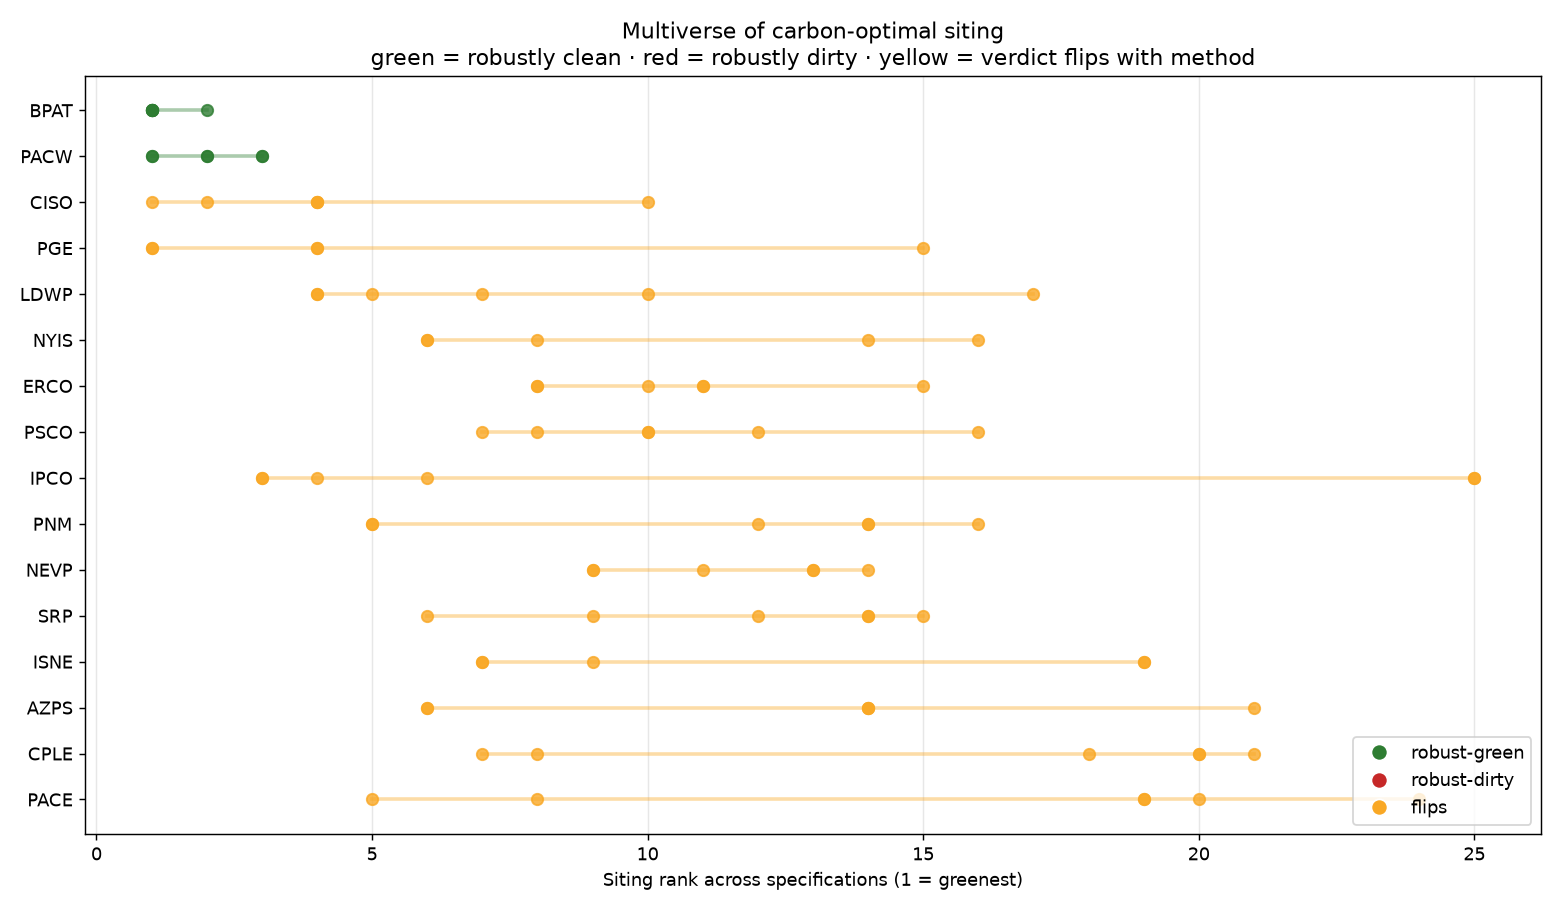
\includegraphics[width=0.92\textwidth]{spec_curve.png}
\caption{Specification-curve (multiverse) of carbon-optimal siting rank. Each row
is a BA; the horizontal spread is its siting rank across the six accounting
specifications (1 = greenest). Green = robust-green (BPAT, PACW), red =
robust-dirty (LGEE), yellow = verdict flips with the accounting choice. Only 3 of
27 BAs are robust.}
\label{fig:spec}
\end{figure}

\section{Discussion}

The carbon-optimal siting recommendation is contingent on the analyst's accounting
choices to a degree that undermines single-metric guidance. The robust policy
signal is narrow---Pacific-NW hydro---and everywhere else the verdict depends on
whether one prices short- or long-run carbon, production or consumption,
BA-average or nodal, and by which estimator. Siting policy and 24/7-CFE
procurement (Ricks, Xu \& Jenkins 2023) should therefore report the accounting
choice explicitly and prefer regions robust across the multiverse. \S5.1 makes
this actionable.

\subsection*{5.1 A decision rule under fragility}

Fragility is not a dead end for a developer; it prescribes two concrete
strategies, both computed from the committed multiverse output.

\paragraph{Rule A---site where the verdict is robust.}
Only BPAT and PACW are green under \emph{every} one of the six accounting choices
(rank ranges 1--2 and 1--3). A recommendation to build there carries no accounting
caveat. Concentrating a carbon-optimal 10~GW build-out in the low-carbon
set---respecting a 20\%-of-local-demand deliverability cap per BA---avoids
\textbf{$\approx$25.2 MtCO\textsubscript{2}/yr (76\%} of the tracked build-out's
marginal emissions) on the production-marginal basis (best site BPAT at 7.4
\kgmwh; \texttt{data/gap.json}). This payoff is itself accounting-dependent---%
\textbf{31.7 MtCO\textsubscript{2}/yr} on the consumption-marginal basis---which
is the point: even the \emph{size of the prize} moves with the accounting choice,
so the robust core is where a developer captures it without betting on which choice
is right.

\paragraph{Rule B---hedge across anti-correlated regions.}
Where the hydro core is unavailable (deliverability, land, water, latency), split
load across a pair of BAs whose rank vectors across the six specifications are
anti-correlated, so the portfolio is insensitive to which accounting choice
ultimately governs. The cleanest case is the temporal axis: \textbf{IPCO} (rank
3--6 short-run, 25 long-run) and \textbf{MISO} (25 short-run, 9 long-run) have a
rank-vector correlation of \textbf{$-0.93$}; a developer able to take the better of
the two under whichever horizon prices the carbon is \textbf{never worse than rank
9}, versus rank 25 for a single-site commitment. On the
production-vs-consumption axis, \textbf{PNM+WACM} (correlation \textbf{$-0.96$})
cap the worst-case rank at 12 versus 25 for WACM alone. (This assumes load can
shift between the paired sites and that the measured anti-correlation persists out
of sample; the correlation is computed over the six specifications, not forecast.)

\section{Limitations}

\begin{itemize}
\item \textbf{Subnetwork truncation (primary exposure).} All results hold
\textbf{within the 27-BA modeled subnetwork}, a truncation of the $\sim$66-BA EIA
interchange network. Flow-tracing (\S3) is solved on this subnetwork, so edges to
unmodeled BAs are cut and imports across them are dropped. This is why the
consumption MEF is \textbf{floored at 0} for solar-saturated, strongly
import-dependent BAs (CISO): with the import edges removed, the raw import-adjusted
estimate dips physically-impossibly negative and is clipped to the non-negative
minimum. \textbf{Direction of bias:} the floor makes such BAs look artificially
clean on the consumption specification, which \emph{widens} their measured rank
range (CISO reaches rank 1 on the consumption spec vs rank 10 on regression MEF).
The truncation therefore, if anything, \textbf{overstates the flip magnitude for
import-dependent BAs}; restoring the omitted (largely fossil) out-of-subnetwork
imports would raise their consumption factors and \emph{narrow} those particular
flips. It does \textbf{not} manufacture the flip---CISO already re-ranks on the
production bases alone---and it does \textbf{not} touch the robust core: BPAT and
PACW are net hydro \emph{exporters}, not import-sensitive. So the central claim (a
small robust set; most BAs contingent) is conservative to this bias, while specific
solar-BA flip magnitudes should be read as upper bounds. A full $\sim$66-BA solve
is the natural next step.
\item \textbf{Short-run vs long-run dependence.} Our short-run MEF is a
dispatch-margin estimate; Cambium LRMER is the long-run build margin. The IPCO
3$\to$25 inversion is driven entirely by this axis, so any headline flip involving
it inherits the short-run/long-run modeling assumptions and is not a single
ground-truth number.
\item \textbf{Cambium scenario dependence.} The long-run results use Cambium's
Mid-case, 2025--2030 vintage. LRMER/SRMER are model- and scenario-dependent; a
different scenario (high-renewable, high-gas) would move the long-run ranks and
could change which BAs invert.
\item \textbf{Nodal estimates are directional only.} The nodal LME is a
congestion-based \emph{index}; an exact nodal \kgmwh{} needs proprietary/CEII shift
factors and offer stacks that are not public. We report spread and direction, not
levels, and there is \textbf{no nodal ground truth} to validate against.
\item \textbf{MEF identification} degrades in storage/solar/import-heavy BAs
(\S4.2; shown, not hidden)---the short-run margin is well-identified in only 6 of
23 BAs.
\item Two-year primary window; longer history (2019--present) only for the 8-BA
subset used in the Holland test.
\end{itemize}

\section{Reproducibility}

All results regenerate from zero via \texttt{gridpulse}
(\texttt{pip install -e ".[prod]"}; \texttt{pytest}; the CLI + \texttt{phase3}
orchestrator). Data sources are public; the only credential is a free EIA API key.
CI runs the live refresh monthly. Cite via \texttt{CITATION.cff} (Zenodo DOI on
release).

\begin{thebibliography}{9}

\bibitem{silerevans2012}
Siler-Evans, K., Azevedo, I.\ L., \& Morgan, M.\ G.\ (2012).
Marginal emissions factors for the U.S.\ electricity system.
\textit{Environmental Science \& Technology}, 46(9), 4742--4748.
\href{https://doi.org/10.1021/es300145v}{doi:10.1021/es300145v}.

\bibitem{dechalendar2019}
de Chalendar, J.\ A., Taggart, J., \& Azevedo, I.\ L.\ (2019).
Tracking emissions in the US electricity system.
\textit{PNAS}, 116(51), 25497--25502.
\href{https://doi.org/10.1073/pnas.1912950116}{doi:10.1073/pnas.1912950116}.

\bibitem{holland2022}
Holland, S.\ P., Kotchen, M.\ J., Mansur, E.\ T., \& Yates, A.\ J.\ (2022).
Why marginal \coo{} emissions are not decreasing for US electricity.
\textit{PNAS}, 119(37), e2116632119.
\href{https://doi.org/10.1073/pnas.2116632119}{doi:10.1073/pnas.2116632119}.

\bibitem{gagnoncole2022}
Gagnon, P., \& Cole, W.\ (2022).
Planning for the evolution of the electric grid with a long-run marginal emission
rate. \textit{iScience}, 25(3), 103915.
\href{https://doi.org/10.1016/j.isci.2022.103915}{doi:10.1016/j.isci.2022.103915}.

\bibitem{ricks2023}
Ricks, W., Xu, Q., \& Jenkins, J.\ D.\ (2023).
Minimizing emissions from grid-based hydrogen production in the United States.
\textit{Environmental Research Letters}, 18(1), 014025.
\href{https://doi.org/10.1088/1748-9326/acacb5}{doi:10.1088/1748-9326/acacb5}.

\bibitem{simonsohn2020}
Simonsohn, U., Simmons, J.\ P., \& Nelson, L.\ D.\ (2020).
Specification curve analysis.
\textit{Nature Human Behaviour}, 4, 1208--1214.
\href{https://doi.org/10.1038/s41562-020-0912-z}{doi:10.1038/s41562-020-0912-z}.

\bibitem{cambium}
NREL Cambium (Gagnon et al.). Long-run marginal emission rates.
\url{https://www.nrel.gov/analysis/cambium.html}.

\bibitem{lme2024}
Steinsultz, N., Christian, P., Cofield, J., McCormick, G., \& Sofia, S.\ (2024).
Validating locational marginal emissions models with wind generation.
\textit{Environmental Research: Energy}, 1(3).
\href{https://doi.org/10.1088/2753-3751/ad72f6}{doi:10.1088/2753-3751/ad72f6}.

\end{thebibliography}

\end{document}
